%%%%%%%%%%%%%%%%%%%%%%%%%%%%%%%%%%%%%%%%%%%%%%%%%%%%%%%%%%
%% HEIG-VD / institut REDS
%%
%% Modèle Latex pour laboratoire
%% 
%% Fichiers à changer : 
%%            - constantes.tex
%%            - Tous les fichiers du corps du rapport 
%%
%% Auteur : MIM
%% Date   : 27.09.2017
%%%%%%%%%%%%%%%%%%%%%%%%%%%%%%%%%%%%%%%%%%%%%%%%%%%%%%%%%%

% Paramétrage du papier utilisé
\documentclass[a4paper,12pt,oneside]{article}

% Ne pas toucher, nécessaire à la mise en forme
\usepackage[utf8x]{inputenc} 
\usepackage[T1]{fontenc} % Nouvelle norme pour codage des caractères
\usepackage{lmodern} % Nouvelle forme de la fonte ComputerModern
\usepackage[frenchb]{babel} % Règles typographiques françaises, césures
\usepackage{graphicx} % Insertion images
\usepackage{float} % Placement exact des figures avec [H]
\usepackage{epstopdf} % Convertir les images eps vers pdf
\epstopdfsetup{outdir=./Images/converted_to_pdf/} % Dossier de sortie des images converties
\usepackage[top=3cm, bottom=3cm, left=3cm, right=3cm, showframe=false]{geometry}
\usepackage{amsmath}
\usepackage[hidelinks]{hyperref} % liens cliquables sans cadre de couleur
\usepackage{pdfpages}
\usepackage{color}
\usepackage{pdflscape} % pages en paysage (annexe du chronogramme du chenillard)
\usepackage{eso-pic} % dessin de l'en-tête et du pied de page tournés sur la page en paysage
\usepackage{booktabs} % traits horizontaux des tableaux (toprule, midrule, bottomrule)
% Pas d'indentation, espace entre les paragraphes (aussi entre les entrées des listes)
\setlength{\parindent}{0pt}
\setlength{\emergencystretch}{3em} % évite les lignes qui débordent dans la marge (noms de signaux longs)
\setlength{\parskip}{1em plus 0.2em minus 0.1em}

% Types de flottants supplémentaires : schémas et chronogrammes, chacun avec sa propre liste
\usepackage{caption}
\captionsetup{labelsep=endash, labelfont=sc} % « FIGURE 1 – ... » comme le style babel français
\addto\captionsfrench{\renewcommand{\tablename}{Tableau}} % « TABLEAU 1 » au lieu de « TABLE 1 »
\usepackage{newfloat}
\DeclareFloatingEnvironment[fileext=los, listname={Liste des schémas}, name=Schéma, placement=H]{schema}
\DeclareFloatingEnvironment[fileext=loc, listname={Liste des chronogrammes}, name=Chronogramme, placement=H]{chronogramme}


% fichier avec les constantes (à adapter pour les étudiants)
%%%%%%%  Constantes (à changer) %%%%%%%%


\newcommand{\nomAuteur}{Noah Missègue}

\newcommand{\titre}{Registre à décalage - Chenillard}

\newcommand{\nbrlabo}{4} % numéro de laboratoire

\newcommand{\prof}{E. Messerli}

\newcommand{\assistant}{Y. Grad}

\newcommand{\classe}{SysLog1-1-A}

\newcommand{\departement}{Technologies industrielles (TIN)}

\newcommand{\cours}{Systèmes Logiques 1 (SysLog1)}


% Entête et pieds de page (A ADAPTER)
\pagestyle{empty}
\usepackage{fancyhdr}
\setlength{\headheight}{27.06pt}
\pagestyle{fancy}
% Entête :
\renewcommand{\headrulewidth}{1pt}
\fancyhead[L]{Labo\nbrlabo: \titre} 
\fancyhead[R]{Rapport de laboratoire} 
% Pied de page
\fancyfoot{} % clear all footer fields
\renewcommand{\footrulewidth}{1pt}
\fancyfoot[R]{Page \thepage} 
\fancyfoot[L]{HEIG-VD | \nomAuteur }

% En-tête et pied de page de la page en paysage (annexe).
% La page est affichée tournée, l'en-tête et le pied de page sont donc dessinés
% tournés de 90° pour être lus dans le même sens que le contenu, avec le même
% texte et les mêmes traits que sur les autres pages.
% Coordonnées sur la feuille portrait : x = 21cm - hauteur en paysage, y = position horizontale en paysage.
\newlength{\largeurPaysage} % largeur du texte sur la page en paysage = hauteur du texte en portrait
\AtBeginDocument{\setlength{\largeurPaysage}{\textheight}}
\newcommand{\enteteEtPiedPaysage}{%
	\thispagestyle{empty}%
	\AddToShipoutPictureFG*{%
		% \smash : la hauteur des éléments ne décale pas leur position une fois tournés
		% en-tête : texte puis trait juste en dessous, à la même distance du bord que sur les pages en portrait
		\put(\LenToUnit{\dimexpr 21cm-18.50cm\relax},\LenToUnit{2.49cm}){\rotatebox{90}{\smash{\makebox[\largeurPaysage][s]{Labo\nbrlabo: \titre\hfill Rapport de laboratoire}}}}%
		\put(\LenToUnit{\dimexpr 21cm-18.35cm\relax},\LenToUnit{2.49cm}){\rotatebox{90}{\smash{\rule{\largeurPaysage}{1pt}}}}%
		% pied de page : trait puis texte
		\put(\LenToUnit{\dimexpr 21cm-1.97cm\relax},\LenToUnit{2.49cm}){\rotatebox{90}{\smash{\rule{\largeurPaysage}{1pt}}}}%
		\put(\LenToUnit{\dimexpr 21cm-1.41cm\relax},\LenToUnit{2.49cm}){\rotatebox{90}{\smash{\makebox[\largeurPaysage][s]{HEIG-VD | \nomAuteur\hfill Page \thepage}}}}%
	}%
}

% debut du corps du rapport 
\begin{document}	
	% première page
	%%%%%%%%%%%%%%%%%%%%%%%%%%%%%%%%%%%%%%%%%%%%%%%%%%%%%%%%
% Ce document ne doit pas être modifié
% Il faut modifier les informations depuis le fichier
% constantes.tex
%%%%%%%%%%%%%%%%%%%%%%%%%%%%%%%%%%%%%%%%%%%%%%%%%%%%%%%%



\begin{center}

\includegraphics[height=2cm]{./images/logo_heig.pdf}
\hfill 
\includegraphics[height=2cm]{./images/logo_hesso.pdf}
\end{center}

\vfill

\begin{center}
	\Large Laboratoire \nbrlabo:\\
	\huge \titre \\
\end{center}


\begin{center}
	\begin{tabular}{l l}
		Département:          & \departement\\
		Unité d'enseignement: & \cours\\
	\end{tabular}
\end{center}


\vfill

%\begin{center}
%	\includegraphics{Images/it.png}
%\end{center}

\vfill

\begin{tabular}{l l}
	\Large	Auteurs:   			  & \Large \nomAuteur\\
	Professeur:           & \prof\\
	Assistant:			  & \assistant\\
	Classe:               & \classe\\
	Salle:                & \salle\\
	Date:                 & \today\\
\end{tabular}

\vfill

\begin{center}

\includegraphics[height=1.5cm]{./images/logo_reds.pdf}
\end{center}
	% enlève le numero sur la premiere page
	\thispagestyle{empty}
	\newpage

	% table des matières et listes, numérotées en chiffres romains (i, ii, iii, ...)
	\pagenumbering{roman}
	\tableofcontents
	\newpage
	\listoffigures
	\listofschemas
	\listofchronogrammes
	\listoftables
	\newpage

	% le corps du rapport commence à la page 1 avec l'introduction
	\pagenumbering{arabic}
	
	% ici débute le corps du rapport
	% changer les sections au cas par cas afin de vous adapter au maximum aux critères
	%\section{Introduction}
	%\section{Analyse et conception}
	%\section{Réalisation et implémentation}
	%\section{Simulation}
	%\section{Conclusion}
	% les méthodologies présentée ci-dessus est une bonne approche pour les petits projets qui ne demandent pas beaucoup de documentation mais n'est pas adaptée à des gros projets où plusieurs personnes vont rédiger de la documentation (Utilisation de git)
	% En modifiant les documents depuis deux endroits différents, si vous répartissez le travail par "thème", chacun va modifier un document et à la fin il suffira de merge ensemble les changements
	\section{Introduction}

Ce laboratoire met en pratique les systèmes séquentiels synchrones vus en cours de SysLog1, et en particulier la décomposition en un bloc combinatoire d'état futur et un registre parallèle/parallèle. Des registres à décalage sont conçus sous Logisim, puis utilisés pour réaliser un chenillard sur 8 LEDs intégré dans la CPLD de la carte MAX\_V\_80P\_25P.

\begin{description}
	\item[Partie 1] Registre à décalage à droite de 4 bits avec enable, réalisé avec 4 bascules D.
	\item[Partie 2] Registre à décalage de 8 bits avec chargement parallèle et décalage à droite/gauche, basé sur un registre parallèle/parallèle.
	\item[Partie 3] Chenillard effectuant une rotation cyclique d'un pattern à droite ou à gauche, testé sur la carte MAX\_V\_80P\_25P.
\end{description}

	\section{Analyse et conception}

\subsection{Partie 1 -- Registre à décalage 4 bits}

Le registre est formé de 4 cellules identiques, une par bit. Chaque cellule contient une bascule D (horloge \texttt{clock\_i}, reset asynchrone \texttt{reset\_i}) précédée d'un multiplexeur 2 vers 1 commandé par \texttt{en\_sh\_i} :
\begin{itemize}
	\item \texttt{en\_sh\_i} = 1 : la cellule reçoit le bit de la cellule de gauche (décalage à droite). La première cellule (bit 3) reçoit \texttt{ser\_r\_i} ;
	\item \texttt{en\_sh\_i} = 0 : la cellule reçoit sa propre sortie Q et conserve son bit.
\end{itemize}
\[
D_n = \overline{\texttt{en\_sh\_i}} \cdot Q_n + \texttt{en\_sh\_i} \cdot Q_{n+1}, \qquad \text{avec } Q_4 = \texttt{ser\_r\_i}
\]

\subsection{Partie 2 -- Registre à décalage 8 bits}

\begin{schema}
	\centering
	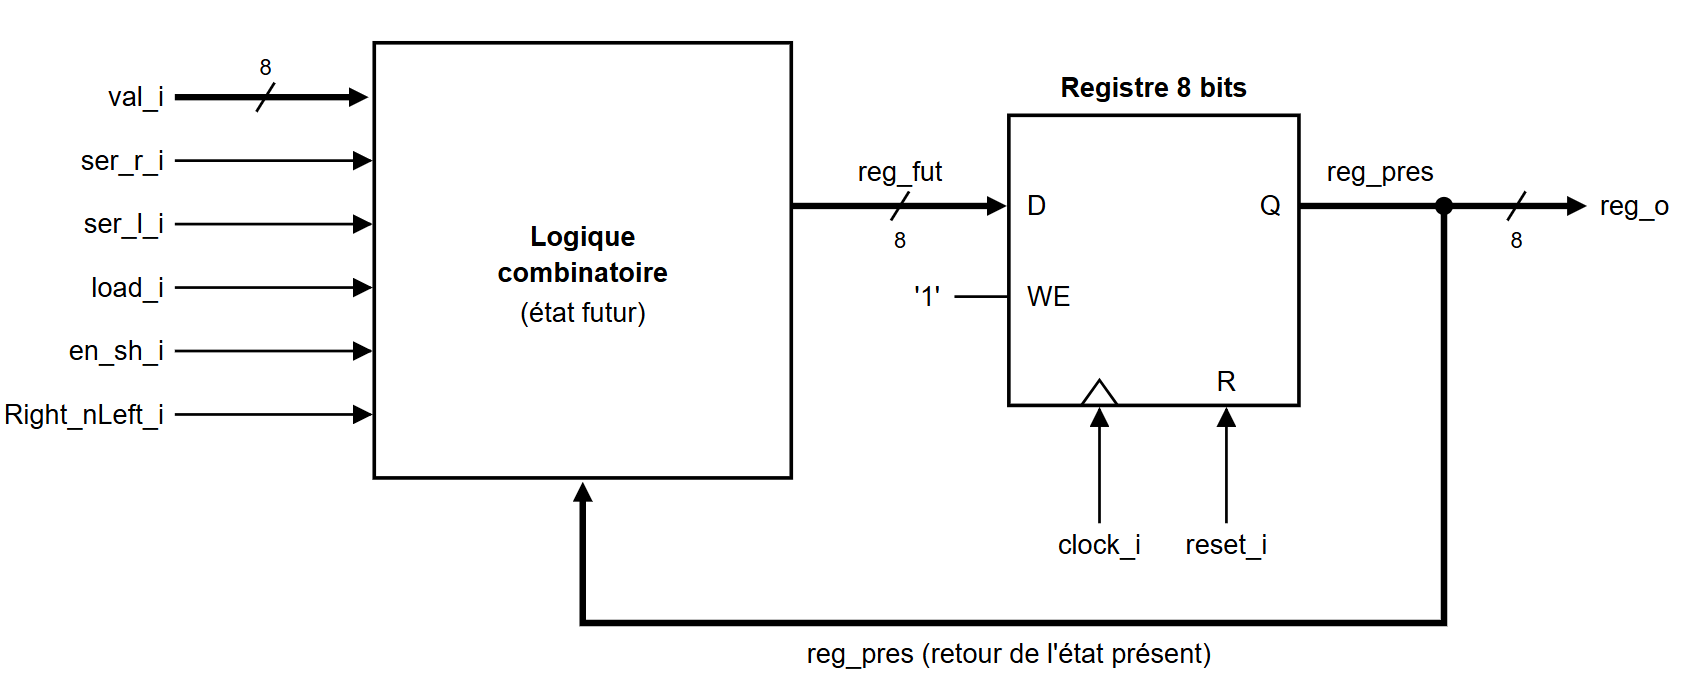
\includegraphics[width=\textwidth]{./images/analyse-partie2.png}
	\caption{Partie 2, schéma bloc, registre à décalage 8 bits}
	\label{fig:analyse_p2}
\end{schema}

Le registre suit la structure d'un système séquentiel synchrone (voir \emph{\underline{Schéma~\ref{fig:analyse_p2}}}) : un bloc combinatoire calcule l'état futur \texttt{reg\_fut} à partir de l'état présent \texttt{reg\_pres} et des commandes, et un registre parallèle/parallèle de 8 bits le mémorise à chaque flanc montant de \texttt{clock\_i}. Son entrée WE est fixée à 1 : le registre est chargé à chaque flanc, c'est donc la logique qui doit recopier \texttt{reg\_pres} lorsque la valeur doit être conservée.

Le bloc combinatoire est décrit par la table des fonctions synchrones (voir \emph{\underline{Tableau~\ref{tab:fonctions_p2}}}), où le cas le plus prioritaire est en haut. Le chargement parallèle passe avant tout le reste, sinon, \texttt{en\_sh\_i} autorise le décalage, dont le sens est donné par \texttt{Right\_nLeft\_i}.

\begin{table}[H]
	\centering
	\small
	\setlength{\tabcolsep}{4.5pt}
	\begin{tabular}{@{}cccll@{}}
		\toprule
		\texttt{load\_i} & \texttt{en\_sh\_i} & \texttt{Right\_nLeft\_i} & \textbf{Fonction} & \texttt{reg\_fut(7..0)} \\
		\midrule
		1 & - & - & Chargement parallèle & \texttt{val\_i(7..0)} \\
		0 & 1 & 1 & Décalage à droite & \texttt{ser\_r\_i \& reg\_pres(7..1)} \\
		0 & 1 & 0 & Décalage à gauche & \texttt{reg\_pres(6..0) \& ser\_l\_i} \\
		0 & 0 & - & Maintien & \texttt{reg\_pres(7..0)} \\
		\bottomrule
	\end{tabular}
	\caption{Partie 2, table des fonctions synchrones, bloc état futur}
	\label{tab:fonctions_p2}
\end{table}

\newpage

\subsection{Partie 3 -- Chenillard}

Le chenillard charge un pattern de 8 bits (\texttt{pattern\_i}, avec \texttt{load\_i}) et le fait tourner d'une position à chaque flanc montant lorsque \texttt{en\_i} = 1, à droite si \texttt{right\_nLeft\_i} = 1, à gauche sinon. La rotation est cyclique : le bit qui sort d'un côté revient de l'autre (voir \emph{\underline{Figure~\ref{fig:exemple_p3}}}).

\begin{figure}[H]
	\centering
	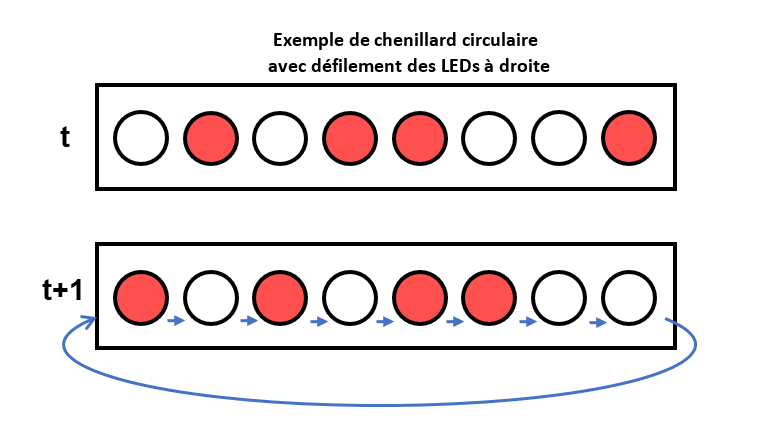
\includegraphics[width=0.7\textwidth]{./images/realisation-partie3-exemple.png}
	\caption{Partie 3, exemple de chenillard circulaire avec rotation à droite (donnée du laboratoire)}
	\label{fig:exemple_p3}
\end{figure}

Le registre de la partie 2 sait déjà charger et décaler. Il suffit donc de reboucler les bits extrêmes sur les entrées série :
\begin{itemize}
	\item \texttt{reg\_o(0)} sur \texttt{ser\_r\_i} : en rotation à droite, le bit 0 revient sur le bit 7 ;
	\item \texttt{reg\_o(7)} sur \texttt{ser\_l\_i} : en rotation à gauche, le bit 7 revient sur le bit 0.
\end{itemize}

	\section{Réalisation}

\subsection{Partie 1 -- Registre à décalage 4 bits}

Le registre est composé de 4 bascules D partageant la même horloge \texttt{clock\_i} et le même reset asynchrone \texttt{reset\_i}. Devant chaque bascule, un multiplexeur commandé par \texttt{en\_sh\_i} sélectionne la donnée à mémoriser : lorsque \texttt{en\_sh\_i} vaut 1, la première bascule reçoit l'entrée série \texttt{ser\_r\_i} et chacune des suivantes la sortie de la bascule précédente. Les sorties des bascules sont regroupées sur le bus \texttt{reg\_o}, la première bascule correspondant au bit de poids fort (bit 3), ce qui réalise un décalage vers la droite.

\begin{schema}
	\centering
	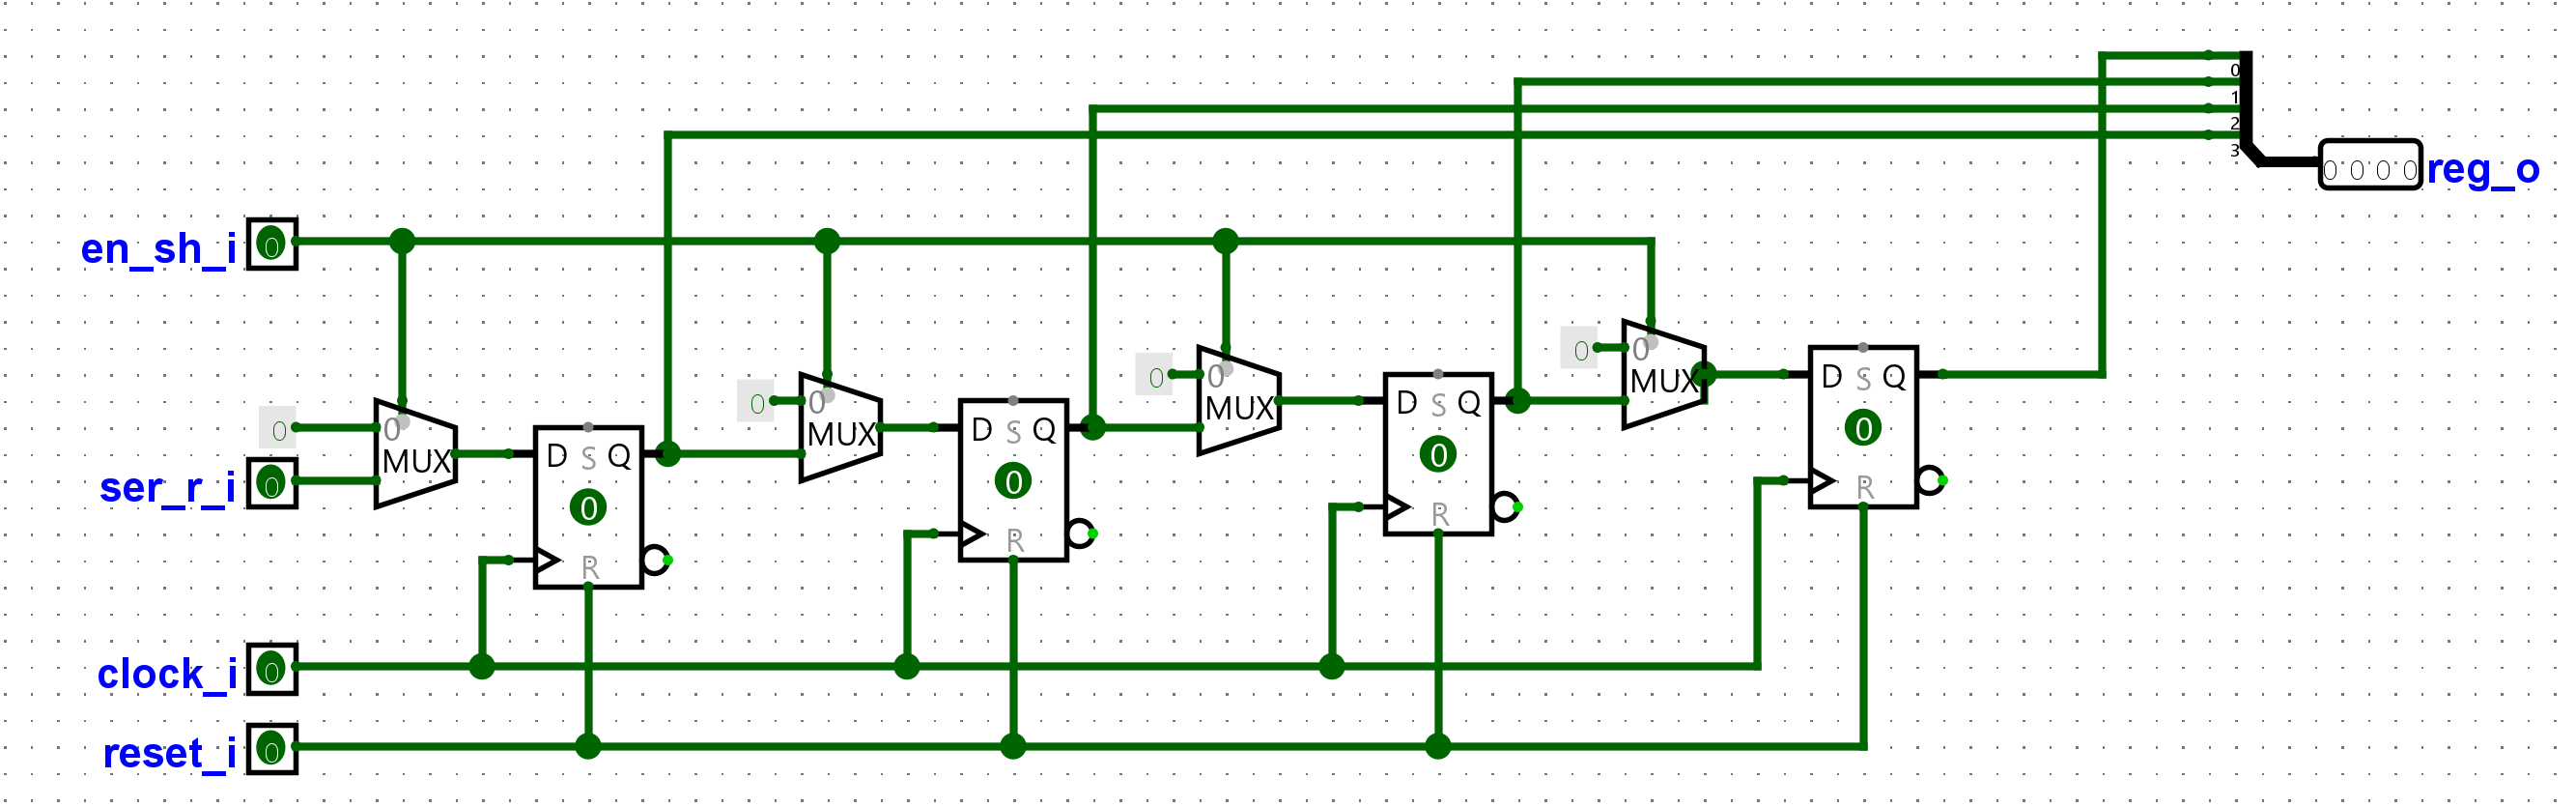
\includegraphics[width=\textwidth]{./images/schema-partie1-logisim.png}
	\caption{Logisim : registre à décalage 4 bits}
	\label{fig:schema_p1}
\end{schema}

\subsection{Partie 2 -- Registre à décalage 8 bits}

% \begin{schema}
% 	\centering
% 	\includegraphics[width=\textwidth]{./images/srg8_ld_sh.png}
% 	\caption{Logisim : registre à décalage 8 bits}
% 	\label{fig:schema_p2}
% \end{schema}

\subsection{Partie 3 -- Chenillard}

% \begin{schema}
% 	\centering
% 	\includegraphics[width=\textwidth]{./images/chenillard.png}
% 	\caption{Logisim : chenillard}
% 	\label{fig:schema_p3}
% \end{schema}

	\section{Simulation}

\subsection{Partie 1 -- Registre à décalage 4 bits}

\begin{figure}[H]
	\centering
	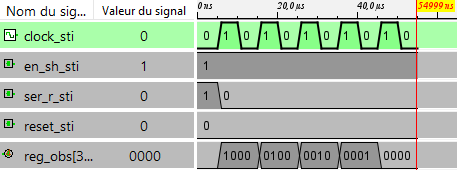
\includegraphics[width=\textwidth]{./images/simulation-partie1.png}
	\caption{Chronogramme de la simulation du registre à décalage 4 bits}
	\label{fig:simu_p1}
\end{figure}

Pour cette simulation, le reset est inactif et le décalage est activé en permanence (\texttt{en\_sh\_sti} = 1). Un 1 est appliqué sur l'entrée série \texttt{ser\_r\_sti} pendant la première période d'horloge, puis l'entrée repasse à 0. On observe sur \texttt{reg\_obs} que ce 1 entre par le bit de poids fort puis se décale d'une position vers la droite à chaque flanc montant de l'horloge : \texttt{1000}, \texttt{0100}, \texttt{0010}, \texttt{0001}, puis \texttt{0000} une fois sorti du registre. Le comportement correspond donc à celui attendu d'un registre à décalage à droite.

\subsection{Partie 2 -- Registre à décalage 8 bits}

% \begin{figure}[H]
% 	\centering
% 	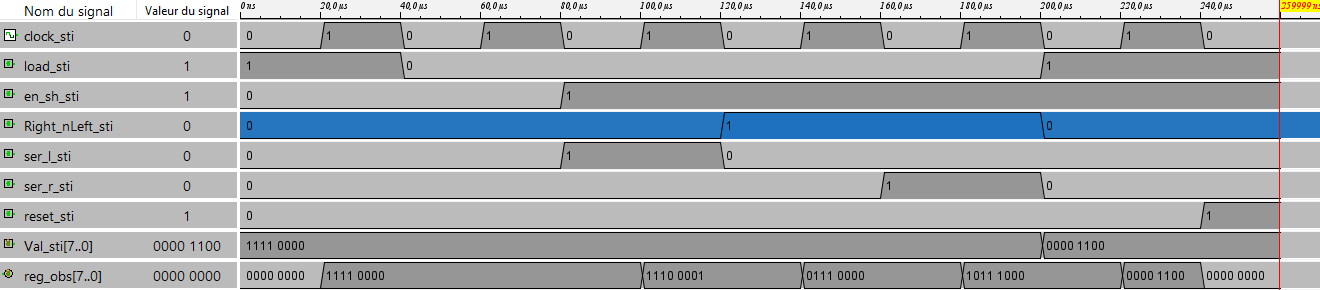
\includegraphics[width=\textwidth]{./images/simulation-partie2.png}
% 	\caption{Simulation du registre à décalage 8 bits}
% 	\label{fig:simu_p2}
% \end{figure}

\subsection{Partie 3 -- Chenillard}

% \begin{figure}[H]
% 	\centering
% 	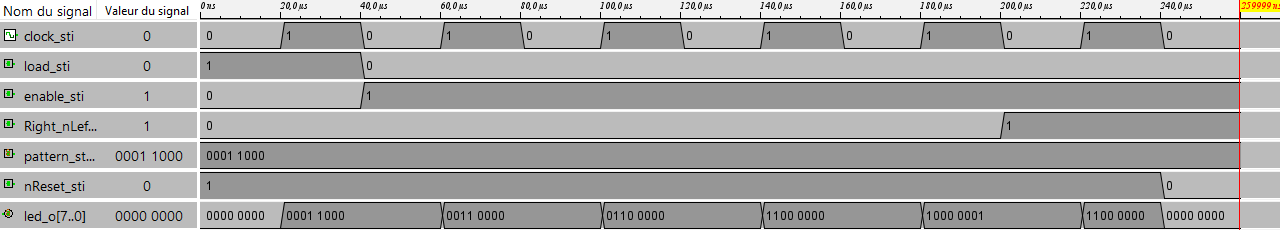
\includegraphics[width=\textwidth]{./images/simulation-partie3.png}
% 	\caption{Simulation du chenillard}
% 	\label{fig:simu_p3}
% \end{figure}

    \section{Intégration et test}

Après la simulation, le chenillard a été intégré depuis le menu FPGA de Logisim, avec la carte \og MAX\_V\_CONSOLE \fg{} comme cible, dans la CPLD MAX V de la carte MAX\_V\_80P\_25P. Le circuit de plus haut niveau utilisé pour l'intégration est \texttt{main}, fourni dans le projet. Il contient le circuit \texttt{chenillard} et relie ses entrées et sa sortie aux boutons, aux interrupteurs, aux LEDs et à l'horloge de la console.

\subsection{Synthèse et vérification du circuit}

L'intégration est lancée depuis la fenêtre Synthesize \& Download (voir \emph{\underline{Figure~\ref{fig:integration_execute}}}). Le circuit \texttt{main} est choisi comme circuit de plus haut niveau (\textit{Toplevel}), la carte \og MAX\_V\_CONSOLE \fg{} comme carte cible et l'action \og Synthesize \& Download \fg{} comme méthode, puis l'exécution est démarrée avec le bouton Execute.

\begin{figure}[H]
	\centering
	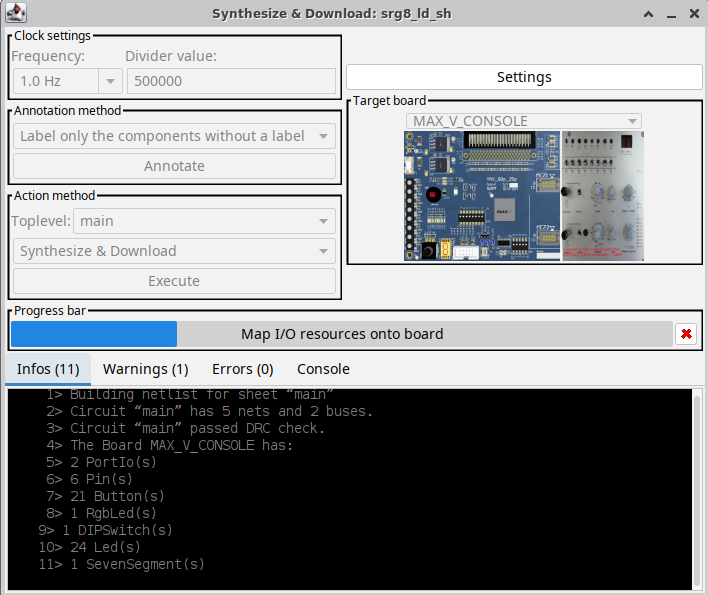
\includegraphics[width=0.6\textwidth]{./images/integration-execute.png}
	\caption{Partie 3, lancement de la synthèse depuis la fenêtre Synthesize \& Download}
	\label{fig:integration_execute}
\end{figure}

Logisim construit d'abord la netlist du circuit \texttt{main}, puis effectue un contrôle des règles de conception (DRC). Les messages de l'onglet Infos montrent que le circuit \og passed DRC check \fg{} et l'onglet Errors n'indique aucune erreur : le circuit est donc valide et peut être synthétisé. Logisim liste ensuite les ressources disponibles sur la carte (boutons, interrupteurs, LEDs, \ldots) et passe à l'étape d'assignation des entrées et sorties, visible dans la barre de progression (\og Map I/O resources onto board \fg{}).

\subsection{Assignation des broches}

Avant la compilation, chaque composant d'entrée et de sortie du circuit \texttt{main} doit être associé à une ressource physique de la carte, selon l'assignation imposée par la donnée du laboratoire :
\begin{itemize}
	\item les commandes \texttt{load\_i}, \texttt{enable\_i} et \texttt{right\_nLeft\_i} sont reliées aux boutons LOAD, EN et R\_nL de la carte MAX V ;
	\item le pattern \texttt{pattern\_i} est réglé avec les 8 interrupteurs S0 à S7 de la console ;
	\item la sortie \texttt{led\_o} est affichée sur les 8 LEDs L0 à L7 de la console ;
	\item l'horloge \texttt{clk\_i} est connectée au signal d'horloge de la console (pin 27a).
\end{itemize}

L'assignation se fait dans la fenêtre Component to FPGA board mapping (voir \emph{\underline{Figure~\ref{fig:integration_mappage}}}) en sélectionnant chaque composant puis la ressource correspondante sur l'image de la carte. Une fois l'assignation terminée, la liste Unmapped Components est vide et tous les composants (\texttt{clk\_i}, \texttt{enable\_i}, \texttt{LED\_0} à \texttt{LED\_7}, \ldots) apparaissent dans la liste Mapped Components. Tous les signaux du circuit sont alors reliés à une ressource de la carte et l'assignation est validée avec le bouton Done.

\begin{figure}[H]
	\centering
	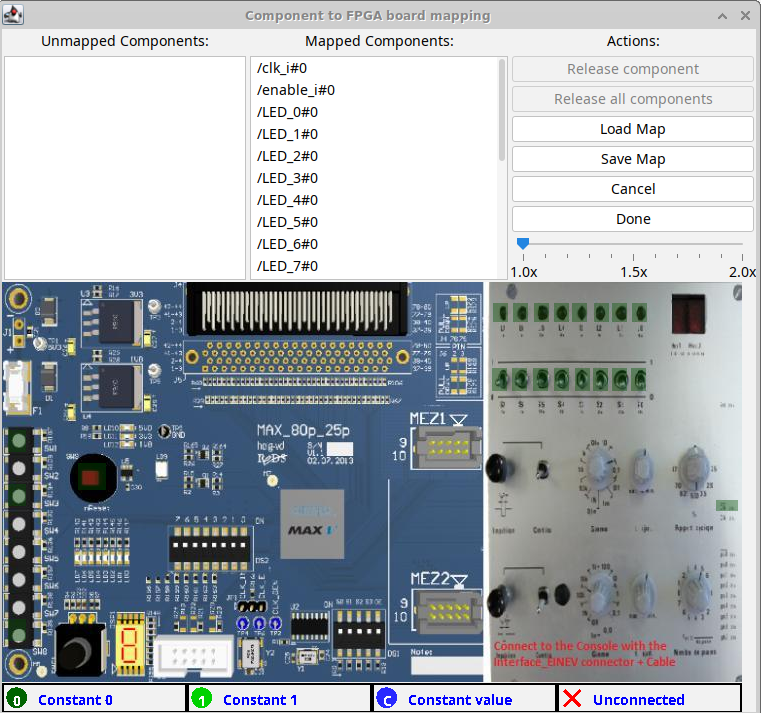
\includegraphics[width=0.6\textwidth]{./images/integration-mappage.png}
	\caption{Partie 3, assignation terminée, tous les composants sont reliés à la carte}
	\label{fig:integration_mappage}
\end{figure}

\subsection{Compilation et programmation}

Une fois l'assignation validée, Logisim génère la description VHDL du circuit, puis Quartus la compile et programme la CPLD de la carte MAX\_V\_80P\_25P par le câble USB-Blaster. La programmation s'est terminée sans erreur et la carte a pu être testée.

\subsection{Test sur la carte}

Une fois la carte programmée, le chenillard a été testé sur le matériel réel. La boîte de commande est connectée au connecteur SUBD25 de la carte MAX V et génère l'horloge du système, réglée à une fréquence de 1 à 4~Hz afin que la rotation du pattern soit visible à l'\oe il nu sur les LEDs. Une LED allumée correspond à un bit à 1. Le montage utilisé est présenté à la \emph{\underline{Figure~\ref{fig:integration_montage}}}.

\begin{figure}[H]
	\centering
	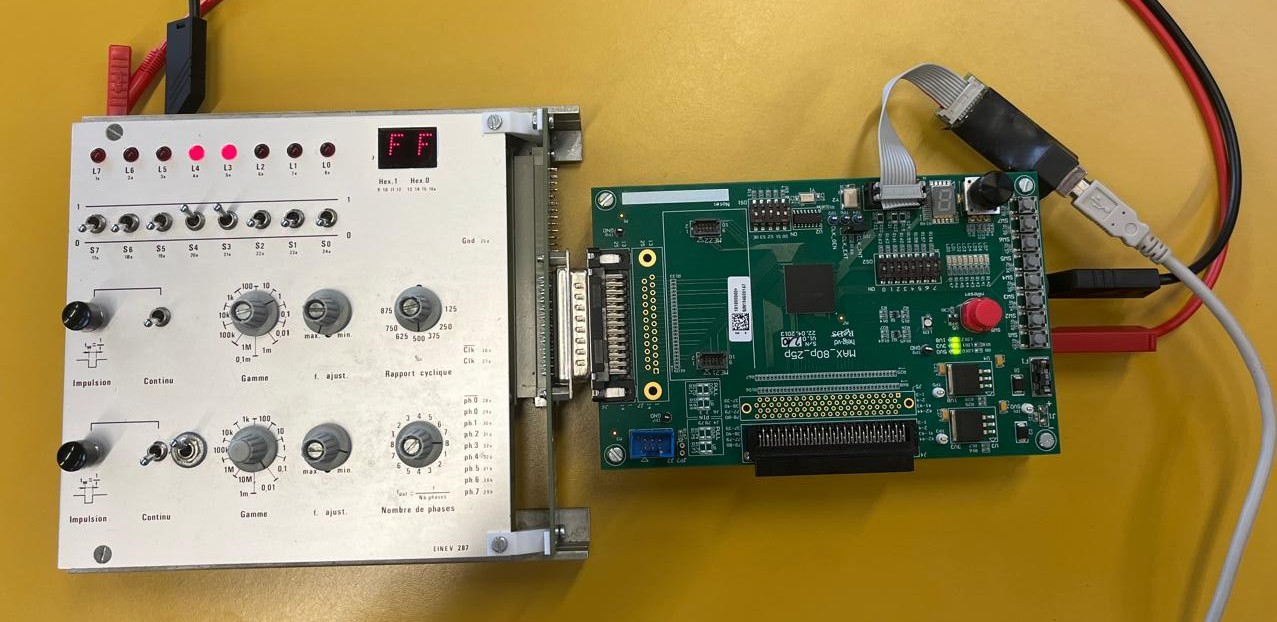
\includegraphics[width=0.6\textwidth]{./images/integration-montage.jpeg}
	\caption{Partie 3, montage de la carte MAX V reliée à la console}
	\label{fig:integration_montage}
\end{figure}

Sur cette photo, la carte MAX V (en bas) est alimentée et programmée par le câble USB-Blaster, et reliée à la console (en haut) par le connecteur SUBD25. Les LEDs L4 et L3 de la console sont allumées, ce qui correspond au pattern \texttt{0001 1000} chargé dans le chenillard, le même que celui utilisé en simulation (voir \emph{\underline{Chronogramme~\ref{fig:simu_p3}}}).

Les tests reprennent chacune des fonctions du chenillard : le chargement d'un pattern avec le bouton LOAD, la rotation à droite et la rotation à gauche avec le bouton EN et le choix du sens avec le bouton R\_nL, l'arrêt de la rotation lorsque EN est relâché, ainsi que le reset. Les résultats sont présentés dans le \emph{\underline{Tableau~\ref{tab:test_carte}}}.

% Remplir avec les résultats observés sur la carte.
\begin{table}[H]
	\centering
	\begin{tabular}{@{}llll@{}}
		\toprule
		\textbf{Commande} & \textbf{LEDs attendues} & \textbf{LEDs obtenues} & \textbf{OK} \\
		\midrule
		Chargement (LOAD) &  &  &  \\
		Rotation à droite (EN, R\_nL = 1) &  &  &  \\
		Rotation à gauche (EN, R\_nL = 0) &  &  &  \\
		Arrêt (EN relâché) &  &  &  \\
		Reset &  &  &  \\
		\bottomrule
	\end{tabular}
	\caption{Partie 3, résultats du test sur la carte}
	\label{tab:test_carte}
\end{table}

Toutes les fonctions testées donnent le résultat attendu. Le comportement du chenillard sur la carte est donc identique à celui observé en simulation.

M. Messerli a validé l'intégration lors de la séance de laboratoire du 27.11.2026.
    
	\section{Conclusion}

Les trois parties du laboratoire ont été réalisées, simulées et, pour le chenillard, testées avec succès sur la carte MAX\_V\_80P\_25P.

\begin{itemize}
	\item \textbf{Partie 1 :} le registre 4 bits décale à droite et conserve sa valeur lorsque \texttt{en\_sh\_i} = 0, grâce au multiplexeur placé devant chaque bascule.
	\item \textbf{Partie 2 :} la table des fonctions synchrones se traduit directement en un multiplexeur d'état futur. La simulation confirme chaque fonction, la priorité du chargement et le reset asynchrone.
	\item \textbf{Partie 3 :} le chenillard réutilise le registre de la partie 2 sans nouvelle logique : reboucler les bits extrêmes sur les entrées série suffit à transformer le décalage en rotation cyclique. Les résultats sur la carte sont identiques à la simulation, et l'intégration a été validée par M. Messerli.
\end{itemize}

Ce laboratoire montre l'intérêt de la décomposition état futur / registre et de la réutilisation : un composant bien conçu et testé sert de base à un système plus complexe avec très peu de modifications.

	
	%Section pour la signature
	\section{Signatures}
  
    Yverdon-les-Bains le \today \\
    \begin{flushright}
  		\nomAuteur
	\end{flushright}
  
	% annexes, numérotées en lettres (A, B, ...)
	% annexes, numérotées en lettres (A, B, ...)
\appendix
% page en paysage pour que le chronogramme du chenillard soit lisible sur une seule page
\begin{landscape}
	\enteteEtPiedPaysage
	\section{Annexes}
	\subsection{Chronogramme de la simulation du chenillard}
	\label{annexe:simu_p3}

	Chronogramme complet de la simulation du chenillard (partie 3), commenté à la section Simulation. Il est découpé en deux parties pour garder une bonne lisibilité.

	\begin{chronogramme}
		\centering
		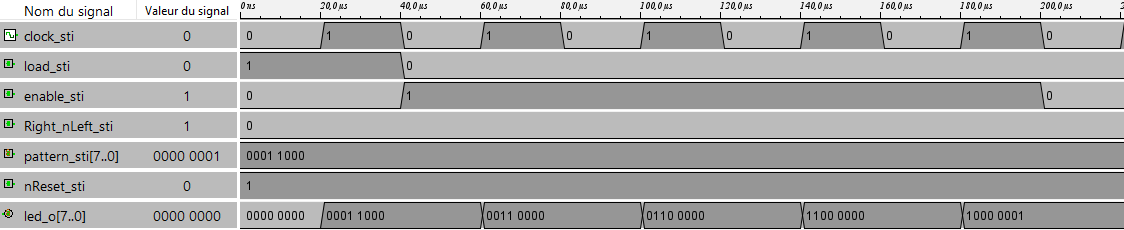
\includegraphics[width=0.85\linewidth]{./images/simulation-partie3-a.png}

		\vspace{0.3cm}
		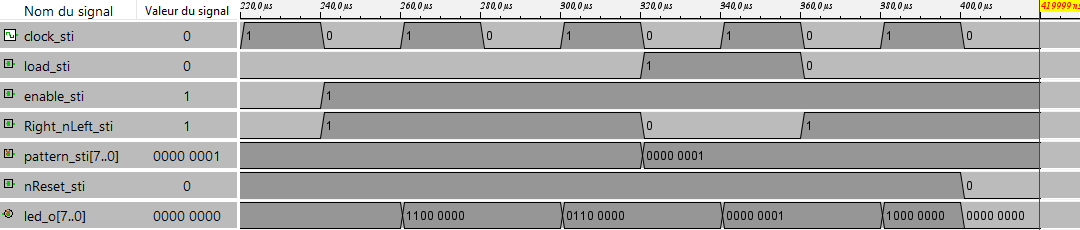
\includegraphics[width=0.85\linewidth]{./images/simulation-partie3-b.png}
		\caption{Partie 3, simulation Logisim, chenillard}
		\label{fig:simu_p3}
	\end{chronogramme}
\end{landscape}

\subsection{Fichier de projet Logisim}
\label{annexe:circ}

Le fichier \texttt{srg8\_ld\_sh.circ} est le fichier de projet Logisim de ce laboratoire. Il est fourni avec ce rapport dans l'archive \texttt{rendu.zip}.


%Fin du document
\end{document}


